\documentclass{standalone}

\usepackage{standalone}
\usepackage{tikz}
\usetikzlibrary{er,positioning, calc}

\begin{document}%
    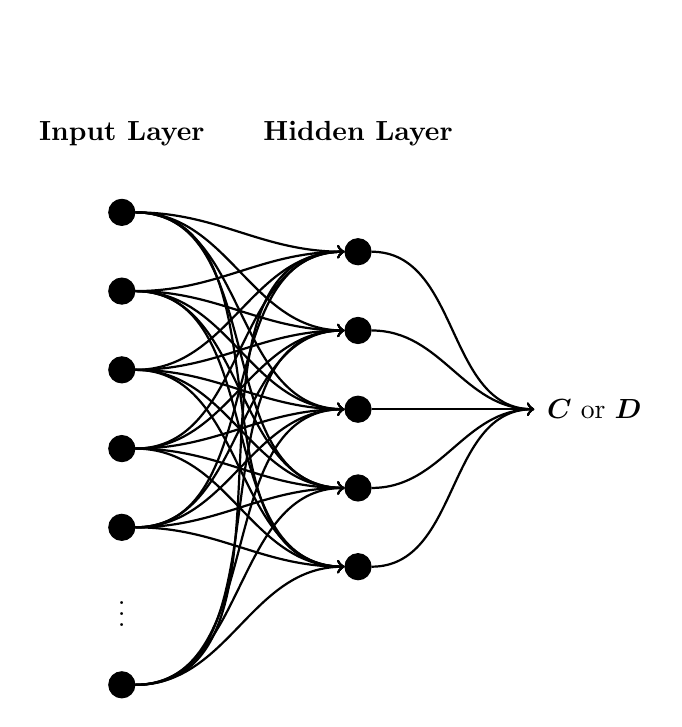
\begin{tikzpicture}%
        \tikzstyle{state}=[minimum width=0.3cm, font=\boldmath];%
        \node[circle] (a) at (0, 1) [state] {\textbf{Input Layer}};

        \node[circle, draw=black, fill=black] (0) at (0, 0) [state] {};
        \node[circle, draw=black, fill=black] (1) at (0, -1) [state] {};
        \node[circle, draw=black, fill=black] (2) at (0, -2) [state] {};
        \node[circle, draw=black, fill=black] (3) at (0, -3) [state] {};
        \node[circle, draw=black, fill=black] (4) at (0, -4) [state] {};
        \node[circle] (5) at (0, -5) [state] {$\vdots$};
        \node[circle, draw=black, fill=black] (6) at (0, -6) [state] {};

        \node[circle] (b) at (3, 1) [state] {\textbf{Hidden Layer}};

        \node[circle, draw=black, fill=black] (0h) at (3, -0.5) [state] {};
        \node[circle, draw=black, fill=black] (1h) at (3, -1.5) [state] {};
        \node[circle, draw=black, fill=black] (2h) at (3, -2.5) [state] {};
        \node[circle, draw=black, fill=black] (3h) at (3, -3.5) [state] {};
        \node[circle, draw=black, fill=black] (4h) at (3, -4.5) [state] {};

        \draw (0) edge[out=0, in=180, ->, thick] node {} (0h);
        \draw (0) edge[out=0, in=180, ->, thick] node {} (1h);
        \draw (0) edge[out=0, in=180, ->, thick] node {} (2h);
        \draw (0) edge[out=0, in=180, ->, thick] node {} (3h);
        \draw (0) edge[out=0, in=180, ->, thick] node {} (4h);

        \draw (1) edge[out=0, in=180, ->, thick] node {} (0h);
        \draw (1) edge[out=0, in=180, ->, thick] node {} (1h);
        \draw (1) edge[out=0, in=180, ->, thick] node {} (2h);
        \draw (1) edge[out=0, in=180, ->, thick] node {} (3h);
        \draw (1) edge[out=0, in=180, ->, thick] node {} (4h);

        \draw (2) edge[out=0, in=180, ->, thick] node {} (0h);
        \draw (2) edge[out=0, in=180, ->, thick] node {} (1h);
        \draw (2) edge[out=0, in=180, ->, thick] node {} (2h);
        \draw (2) edge[out=0, in=180, ->, thick] node {} (3h);
        \draw (2) edge[out=0, in=180, ->, thick] node {} (4h);

        \draw (3) edge[out=0, in=180, ->, thick] node {} (0h);
        \draw (3) edge[out=0, in=180, ->, thick] node {} (1h);
        \draw (3) edge[out=0, in=180, ->, thick] node {} (2h);
        \draw (3) edge[out=0, in=180, ->, thick] node {} (3h);
        \draw (3) edge[out=0, in=180, ->, thick] node {} (4h);

        \draw (4) edge[out=0, in=180, ->, thick] node {} (0h);
        \draw (4) edge[out=0, in=180, ->, thick] node {} (1h);
        \draw (4) edge[out=0, in=180, ->, thick] node {} (2h);
        \draw (4) edge[out=0, in=180, ->, thick] node {} (3h);
        \draw (4) edge[out=0, in=180, ->, thick] node {} (4h);

        \draw (6) edge[out=0, in=180, ->, thick] node {} (0h);
        \draw (6) edge[out=0, in=180, ->, thick] node {} (1h);
        \draw (6) edge[out=0, in=180, ->, thick] node {} (2h);
        \draw (6) edge[out=0, in=180, ->, thick] node {} (3h);
        \draw (6) edge[out=0, in=180, ->, thick] node {} (4h);

        \node[circle] (e) at (6, -2.5) [state] {$C$ or $D$};
        \draw (0h) edge[out=0, in=180, ->, thick] node {} (e);
        \draw (1h) edge[out=0, in=180, ->, thick] node {} (e);
        \draw (2h) edge[out=0, in=180, ->, thick] node {} (e);
        \draw (3h) edge[out=0, in=180, ->, thick] node {} (e);
        \draw (4h) edge[out=0, in=180, ->, thick] node {} (e);
    \end{tikzpicture}
\end{document}